% !TeX root = ../main.tex
\subsection{Chromatin as the information center of a cell} \label{intro: chromatin}

\begin{wrapfigure}{r}{0.45\textwidth}
    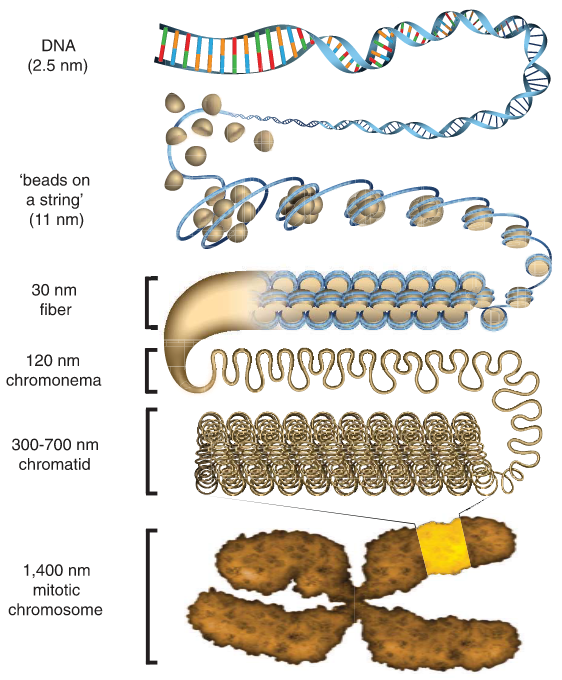
\includegraphics[width=\textwidth]{./images/HierarchicalDNA.png}
    \caption{Image representing the hierarchical compaction of DNA in subsequently more compact and dense fibers.}
    \label{fig: chromatin compaction}
\end{wrapfigure}

All the living organisms have, inside the nucleus, the largest portion of their DNA, which is the main molecule through which information is passed from the old generations to the daughter cells. Due to the extreme length of the chromosomes, an assembly of DNA, proteins and RNA, called chromatin, is built in a necessary ordered and functional manner
\cite{paroBiologyChromatin2021}. 
The most important proteins used to reach this scope are the histones, towards which DNA is wrapped around, forming the nucleosomes. To govern the functioning of the DNA, the histones and the nucleic acid itself are subjected to a variety of modifications, such as methylation. The latter alteration, in mammals, occurs in specific sites of the genome, called CpGs, where a cytosine is connected directly to a guanine. Methylations of regulatory elements have been implicated in determining cell identity and chromatin structure
\cite{liauAdaptiveChromatinRemodeling2017, shareefExtendedrepresentationBisulfiteSequencing2021}. 
Among the proteins that interact with the DNA, CTCF is one of the most important to be mentioned. It is a protein conserved in eukaryotes and is ubiquitous in mammalians
\cite{kimCTCFMultifunctionalProtein2015a}, 
and contains a Zinc-finger that binds to the DNA. The act of binding is performed in cooperation with cohesins, and causes the folding of the chromatin.
\cite{hsiehEnhancerPromoterInteractions2022,kimCTCFMultifunctionalProtein2015a}.\\

When it comes to its structure, the DNA is thought to fold in a hierarchical manner, as depicted in figure \ref{fig: chromatin compaction}.
However, this hypothesis makes a simplification: the fibers could have a range of diameters which depend on their activity and their location.
\cite{ouChromEMTVisualizing3D2017a,robinsonEMMeasurementsDefine2006}.
Importantly, the diameter of the nucleosomes was determined to be, on average, equal to $10$ nm. This type of measure was taken into account when building the Fine Scale (FS) model (chapter \ref{chap: the model description}).
